% Template for ICASSP-2016 paper; to be used with:
%          spconf.sty  - ICASSP/ICIP LaTeX style file, and
%          IEEEbib.bst - IEEE bibliography style file.
% --------------------------------------------------------------------------
\documentclass{article}
\usepackage{spconf,amsmath,graphicx,float}

% Example definitions.
% --------------------
\def\x{{\mathbf x}}
\def\L{{\cal L}}

% Title.
% ------
\title{Title Report}
%
% Single address.
% ---------------
\name{Atom Group: Jifu Zhao (jzhao59), Jinsheng Wang ()}
\address{Nuclear, Plasma, and Radiological Engineering \\
              University of Illinois at Urbana-Champaign\\
		       Urbana, Illinois 61801, USA}

\begin{document}
%\ninept
%
\maketitle

\section{Introduction}

\section{Pre-rocessing}

\section{Methods}

\subsection{Simple Linear Regression}

\subsection{Lasso Regression}


%\begin{figure}[htb]
%\centering
%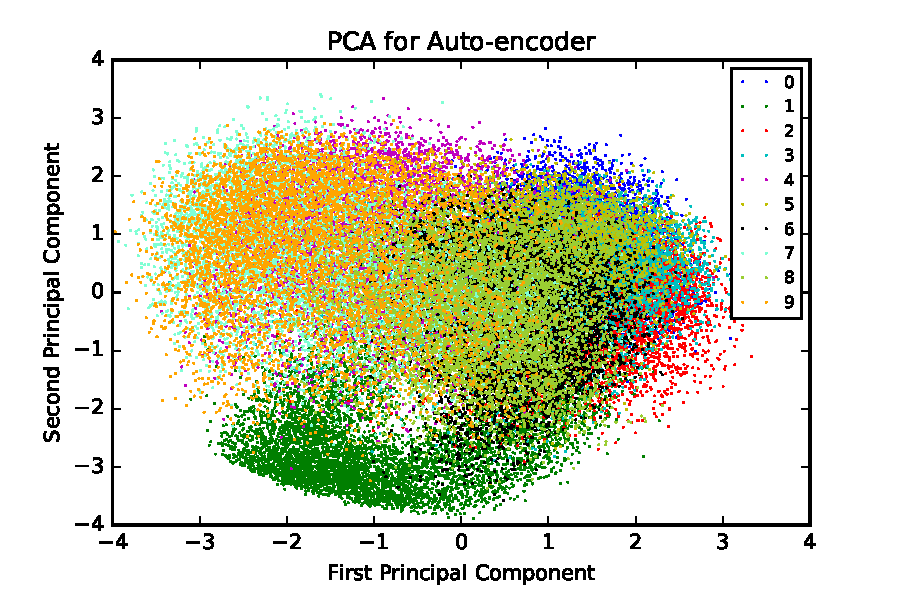
\includegraphics[width=8.5cm]{./figures/autoencoder.pdf}
%\caption{Illustration of auto-encoder system.}
%\label{fig:autoencoder}
%\end{figure}


\section{Conclusions}
\label{sec:conclusion}


\subsection*{Acknowledgement}
\label{sec:acknowledgement}

The authors would like to thank Xichen Huang for his tutorial notebook in Piazza.

\vfill\pagebreak

% References should be produced using the bibtex program from suitable
% BiBTeX files (here: strings, refs, manuals). The IEEEbib.bst bibliography
% style file from IEEE produces unsorted bibliography list.
% -------------------------------------------------------------------------
\bibliographystyle{IEEEbib}
%\bibliography{strings,refs}
\bibliography{strings}

\end{document}
